\chapter{Kolaboratívny editor}

\label{kap:zdialtelnost} % id kapitoly pre prikaz ref

Myšlienka kolaboratívneho editora bola prvýkrát zaznamenaná už v roku 1968 Douglasom Engelbartom. 
Do popularity sa však dostala až nedávno, približne 20 rokov od prvého záznamu.
Kolaboratívny editor umožňuje viacerým používateľom naraz upravovať jeden dokument.
Tieto editory sa rozdeľujú na dve kategórie podľa typu aplikovania úprav:
\begin{itemize}
  \item v reálnom čase - zmeny dokumentu sa okamžite zobrazia všetkým používateľom
  \item s oneskorením - zmeny dokumentu sa nedejú okamžite (podobne ako pri ver --- zionovacích
  systémoch ako Git, Mercurial)
\end{itemize}
V bakalárskej práci sa zaoberáme editormi so zmenami, ktoré aplikujú úpravy v reálnom čase, kde treba
riešiť synchronizáciu editorových inštancií používateľov a riešenie možných konfliktov.

Problematika kolaboratívnych editorov v reálnom čase sa dá rozdeliť do samostatných zmysluplných 
podkapitol
\begin{itemize}
\item  technické výzvy
\item  algoritmy riešiace konkurentné modifikácie jedného dokumentu
\end{itemize}

\section{Technické výzvy}
Technické výzvy pramenia z asynchrónnej komunikácie po sieti. Teoreticky, keby táto 
komunikácia bola okamžitá, vytvorenie takéhoto editora by nebolo veľmi odlišné od
editora pre jedného používateľa. Algoritmus\label{algo:nesubezne_editovanie}, 
riešiaci takýto problém by mohol fungovať na základe 
\textit{upravovacieho zámku}. Fungoval by celkom jednoducho:
\begin{enumerate}
  \item Požiadanie servera o \textit{upravovací zámok}
  \item Počkanie na schválenie zo servera, že sme na rade s úpravou
  \item Úprava dokumentu
  \item Vzdanie sa \textit{upravovacieho zámku}
\end{enumerate}
Keďže komunikácia so serverom je okamžitá, tak všetci používatelia by v čase modifikácie
dokumentu mali rovnaký obsah dokumentu. 

Avšak rýchlosť komunikácie je obmedzená latenciou siete. To vytvára základnú dilemu: 
používatelia potrebujú okamžite vidieť vlastné úpravy, ktoré sú do dokumentu zapracované,
ale ak sú začlenené okamžite, tak pre latenciu komunikácie musia byť ich
úpravy nevyhnutne vložené do rôznych verzií dokumentu.

Jednou s možností by mohlo byť zamedzenie konkurentných úprav dokumentu (algoritmus by bol podobný
\ref{algo:nesubezne_editovanie}). To však vytvára zbytočné podmienky na architektúru riešenia,
pretože treba vytvorť mechanizmus, ktorý zabezpečuje, že dokument upravuje najviac jeden
používateľ. Taktiež to vytvára zbytočné obmedzenia pre používateľov, pretože nemôžu naraz
upravovať daný dokument (musia sa striedať).

Ďalšou, pre používateľa príjemnejšou, voľbou je optimistická
replikácia, kde sa zmeny v dokumente uplatňujú postupne a prípadné chyby a nekonzistentnosti sa
riešia neskôr. Neskôr v texte ukážeme, že existuje spôsob akým docieliť konkurentné úpravy 
dokumentu zaručene bez konfliktov. Takýto algoritmus je popísaný v kapitole \ref{kap:cdrt}.

Obmedzíme sa teraz iba na textový editor. Aj keď algoritmus, ktorý neskôr v texte ukážeme, je
všeobecnejší a fungoval by aj pre iné typy editorov podporujúce zdieľanie iných entít, napríklad
obrázkov, rôznych variantov textu... 

\medskip

Problém súbežnej modifikácie jedného textového dokumentu je, že jednoduché textové operácie ako
pridať alebo zmazať znak, nie sú komutatívne \ref{obr:nekomutativita} a ani 
idempotentné \ref{obr:neidempotentnost}. Keďže používatelia
modifikujú dokument cez sieť, nie je zaručené v akom poradí sa modifikácie uskutočnia. 
Ilustrujme tieto problémy na príklade:

\begin{figure}[H]
\centerline{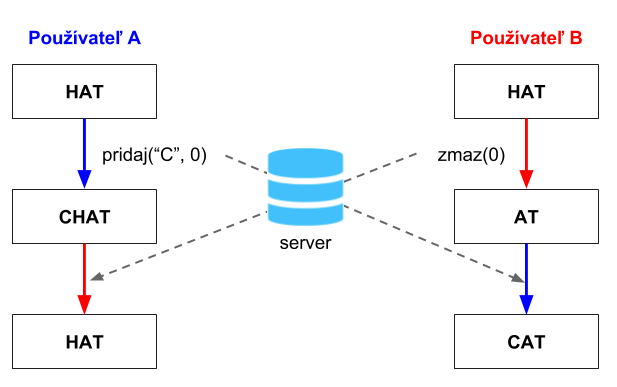
\includegraphics[width=0.6\textwidth]{images/nekomutativne_operacie}}
\caption[Nekomutativita textových operácii]{Nekomutativita textových operácii}
\label{obr:nekomutativita}
\end{figure}

\begin{figure}[H]
\centerline{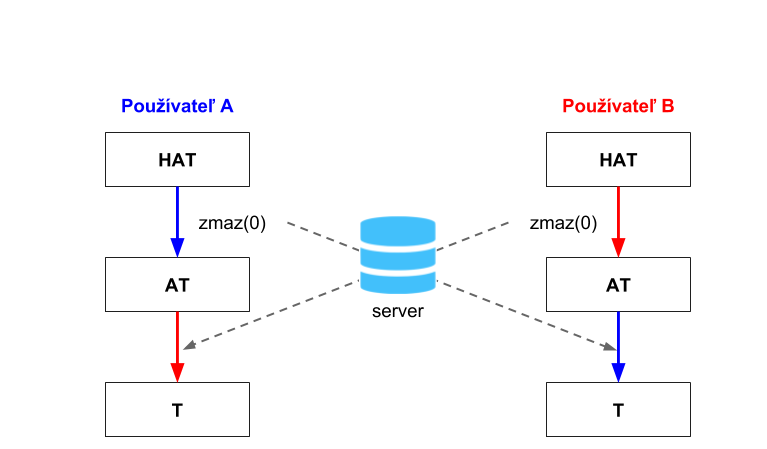
\includegraphics[width=0.6\textwidth]{images/neidempotentne_operacie}}
\caption[Neidempotentnosť textových operácii]{Neidempotentnosť textových operácii}
\label{obr:neidempotentnost}
\end{figure}

% TODO: prepis ma
Výzvou v spolupráci v reálnom čase je nájsť spôsob, akým možno aplikovať úpravy od vzdialených
používateľov, ktoré boli pôvodne vytvorené vo verziách dokumentu, nikdy lokálne neexistovali a môžu
byť v rozpore s vlastnými miestnymi úpravami používateľa. 

Najsofistikovanejšie riešenia vyriešia tento problém spôsobom, ktorý nevyžaduje server, nepoužíva
uzamknutie (všetci používatelia môžu voľne upravovať všetky časti dokumentu súčasne) a podporuje
ľubovoľný počet používateľov (obmedzený iba zdrojmi počítačov). Tento prístup využíva napríklad
\textit{SubEthaEdit}, ktorý je však dostupný iba pre operačné systémy macOS a využíva
technológie ako \cite{bonjour}, ktoré sú špecifické pre tento operačný systém. Viac sa o
existujúcich programoch podporujúcich kolaboratívne úpravy dozvieme v kapitole
\ref{kap:usability_and_similar}.

Pri klient-server riešení je pri otvorení dokumentu priradená jednej z inštancií editora
úloha servera. Tento server zaisťuje, že ostatné editory sú synchronizované. Pri každej zmene
dokumentu inými používateľmi server obdrží upozornenia na vykonané zmeny, pričom zaistí, aby
sa tieto zmeny aplikovali aj u ostatných používateľov. 
V niektorých modeloch sa zmeny na klientovi neodzrkadľujú dovtedy,
kým sa zo servera nevráti odpoveď, že dané zmeny boli aplikované u všetkých používateľov.
Príkladom takéhoto editora je editor \textit{Gobby}. Tieto riešenia sú 
jednoduchšie na implementáciu, ale používateľov výrazne obmedzujú. Ak je latencia siete
príliš vysoká, používateľ musí dlho čakať.

My sme sa v bakalárskej práci rozhodli použiť klient-server model, pričom za synchronizáciu klientov
je zodpovedný výhradne server. Podobný prístup používa napríklad spoločnost Google v 
niektorých ich produktoch.

\section{Algoritmy riešiace konkurentné modifikácie}
Na riešenie synchronizácie klientov existujú dva dobre preskúmané typy algoritmov:
\begin{enumerate}
  \item OT - Prevádzková transformácia \textit{(angl. Operational transformation)}
  \item CRDT - Bezkonfliktné replikovateľné dátové typy 
  \textit{(angl. Conflict-free replicated data type)}
\end{enumerate}

V bakalárskej práci použijeme typ CRDT, pretože typ OT je teoretický model, ktorý predchádza typu CRDT a v praxi
je jeho implementácia veľmi náročná a často nefunguje tak dobre, ako je spomínané v teórii.
Taktiež použitie typu OT je vo väčších projektoch neškálovateľné \cite{ot_nonscalable}. 
